\section{Background}

\label{sec:background}

\subsection{Attendance Tracking Systems}

Many technology-enhanced attendance tracking systems have been proposed, but
each has certain drawbacks that make it non-ideal for classroom attendance
tracking applications (Table~\ref{tab:existing-solutions}). We explore proposed
solutions in greater depth below.

\subsubsection{Biometric}

Biometrics are an enticing solution that provide strong authentication and
confidence in user identity. However, biometrics require that users be in close
proximity to a central device to record biometric information and/or they
require that users possess specialized biometric scanners that are not widely
commercially available. The necessity of close proximity to a relatively rare
scanner can lead to large queues as students wait to scan their biometric
information if a central biometric device is the chosen solution.

\subsubsection{iClicker}

Another solution that attempts to overcome the challenge of limited proximity
while maintaining strong authentication are iClickers~\cite{iclicker}. These
devices are widely used in academia and are registered to specific students to
form a 1-1 mapping of student to iClicker. The student can then check into a
centralized attendance recording device with their iClicker to notify the
instructor of their attendance. However, the iClicker is another excess piece
of hardware that the student must carry on their person at all times and has
non-negligible cost that is typically placed upon students who  must purchase
or rent the devices. Additionally, iClickers fall victim to the assumption that
students will not simply give their device to another student to check in for
them.

\subsubsection{RFID}

RFID is an intriguing solution that can provide a 1-1 mapping of student to
device, similar to an iClicker, while being much cheaper than the iClicker
solution. However, RFID is similarly susceptible to the issues mentioned
previously with biometrics and iClickers. RFID requires excess hardware for
students to carry with them, requires additional RFID scanners, requires close
proximity to a check in point, and RFID identity can easily be shared by simply
sharing one’s RFID hardware.

\subsubsection{Web Application}

Alternatively, web and Wi-Fi based solutions provide no need for additional
hardware infrastructure as most users do have access to a device with web and
Wi-Fi access. However, these solutions require reliable Wi-Fi or mobile data
connection in order to operate between a user's web device and centralized
attendance tracking system. Not only can a reliable connections not always be
guaranteed, but device authenticity also suffers in this approach as spoofing a
device’s identity over Wi-Fi connection is trivial. Additionally, these
solutions that rely on Wi-Fi connection require an extensive amount of overhead
in associating with an access point every time that the user authenticates to
the attendance tracking solution. These challenges facing web and Wi-Fi based
solutions make these approaches unsuitable for unreliable environments and
scenarios that require strong authentication of a user’s identity such as the
proposed classroom attendance tracking.

\begin{table} \centering \begin{tabularx}{\columnwidth}{lX} \toprule Proposed
Solution & Issues \\ \midrule Biometrics & Close proximity, excess hardware \\
iClicker & Trivial identity sharing, excess hardware \\ RFID & Trivial identity
sharing, close proximity, excess hardware \\ Web Application & Reliable
connection required, identity spoofing, high overhead \\ \bottomrule
\end{tabularx} \caption{Existing solutions and their shortcomings for classroom
attendance tracking} \label{tab:existing-solutions} \end{table}


\subsection{Bluetooth Low Energy}

\begin{figure} \centering
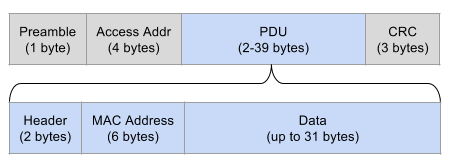
\includegraphics[width=\columnwidth]{figures/ble-packet.png} \caption{BLE
advertising beacon packet structure with up to 31 bytes user data}
\label{fig:ble-packet} \end{figure}

Bluetooth is a close-range wireless communication protocol that was first
develop in 1994 by the telecom company Ericsson. Over time, Bluetooth has
become ubiquitous for many applications (over 4 billion devices shipped in
2014~\cite{bluetooth-2014-annual-report}). However, in light of recent interest
in the Internet of Things (IoT) and related low power sensor networks, classic
Bluetooth's (version < 4.0) high energy consumption and complex pairing
mechanism have become major limitations to Bluetooth's continued adoption.
Thus, BLE was incorporated into Bluetooth in 2010. These changes have opened up
a whole new class of uses and spurred rapid growth -- most modern mobile phones
ship with BLE functionality and usage is expected to reach 60 million devices
by 2019~\cite{beacon-shipment-projection}. This is a key determining factor in
our selection of BLE as the wireless technology of choice. BLE is already
available on most laptops and mobile devices today, and the cost of BLEATS
deployments will continue to decrease as BLE technology becomes more and more
ubiquitous. 

\begin{figure} \centering
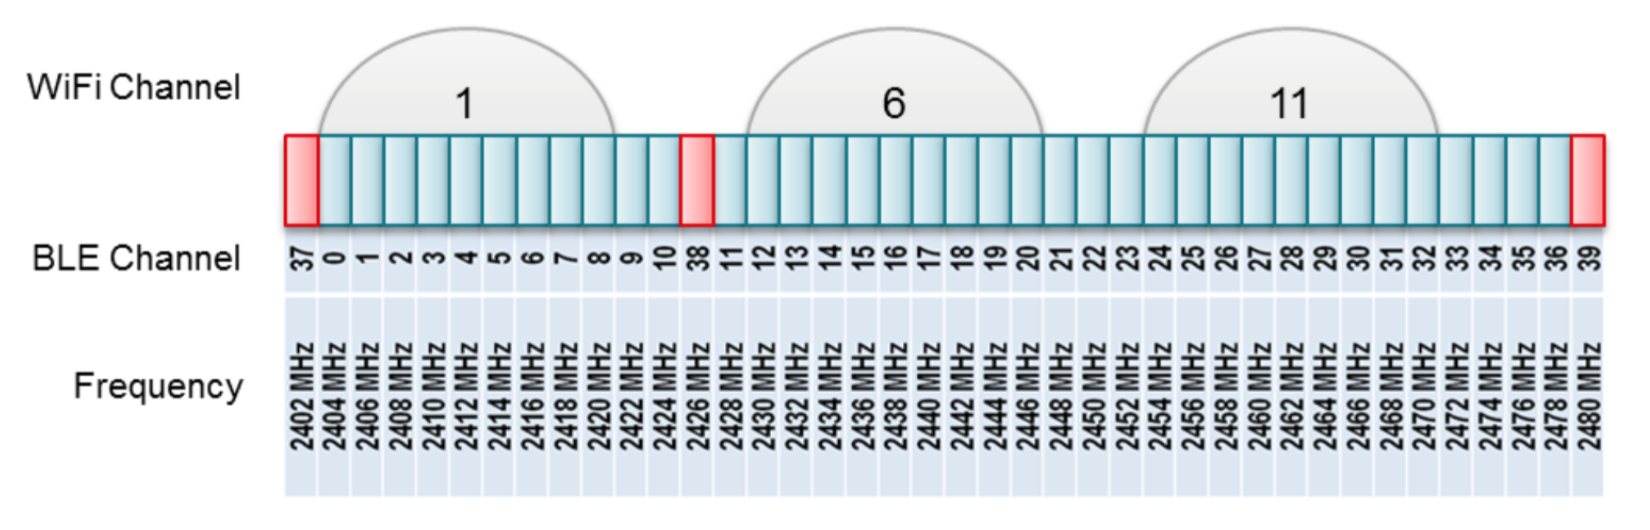
\includegraphics[width=\columnwidth]{figures/ble-wifi-coexistence.png}
\caption{Overlap between BLE and WiFi 802.11 channels}
\label{fig:ble-wifi-coexistence} \end{figure}

BLE modifies Bluetooth Classic by simplifying data transfer into a
connection-less beacon protocol that enables basic fixed-size advertising tags
(Figure~\ref{fig:ble-packet})  to be sent periodically, either for service
discovery or short data transfer. These advertising tag beacons operates on
three reserved channels within the Bluetooth 2400-2483.5 MHz spectrum,
specifically channels 37, 38, and 39. Multiple channels are used to avoid
overloading a single channel, but the number of channels is limited to three in
order to limit long beacon scanning/discovery times across a larger number of
channels. The channels 37, 38, and 39 are also specifically chosen to
complement and coexist with the main channels used in 802.11 Wi-Fi connections
(Figure~\ref{fig:ble-wifi-coexistence}). This is an especially useful property
for BLEATS since most classroom environments contain strong WiFi signaling for
educational use that would otherwise interfere with the majority of BLE
channels.

BLE supports two modes for transferring data: passive and active. In both
modes, initial beacon packets, which can support up to 31 bytes of user data,
are transmitted serially across all three channels based on a specified
advertising interval that is typically 100 milliseconds to 1 second. In passive
mode, receivers simply listen for the beacon and process the data without
sending a response, so senders using passive mode can immediately become
inactive until the next advertising interval. Active mode, on the other hand,
is meant to be used used when the receiver requires more data than the 31 bytes
included in the initial advertisement tag. In active mode, upon packet
reception, the receiver sends an immediate SCAN\_REQ response for more
information, which triggers a SCAN\_RSP from the sender with the additional
data. Senders in active mode cannot immediately become inactive after
transmission because they must wait for potential responses asking for more
data. This leads to higher energy consumption than passive mode. 

For BLEATS, we exclusively utilize and evaluate passive mode communication
because we do not require more data than the 31 bytes sent in the initial
beacon packet, and value the lower energy consumption that passive mode
affords. Additionally, previous work has also demonstrated the poor scalability
of active mode BLE transmission~\cite{robin-ble}, making active mode BLE
communication even less suitable for BLEATS.




